\documentclass[12pt,a4paper]{report}

% --- Packages ---
\usepackage[utf8]{inputenc}
\usepackage[T1]{fontenc}
\usepackage{lmodern} % Better font for technical docs
\usepackage{graphicx}
\usepackage{hyperref}
\usepackage{geometry}
\usepackage{titlesec}
\usepackage{listings}
\usepackage{xcolor}
\usepackage{booktabs}
\usepackage{float}
\usepackage{enumitem}
\usepackage{microtype}
\usepackage{caption}

% TikZ for native LaTeX diagrams
\usepackage{tikz}
\usetikzlibrary{shapes.geometric, arrows.meta, positioning, fit, calc, backgrounds}

% --- Layout & Colors ---
\geometry{a4paper, margin=1in}

\definecolor{primary}{RGB}{79, 70, 229} % Indigo-600
\definecolor{secondary}{RGB}{16, 185, 129} % Emerald-500
\definecolor{codegray}{rgb}{0.5,0.5,0.5}
\definecolor{codepurple}{rgb}{0.58,0,0.82}
\definecolor{backcolour}{rgb}{0.96,0.96,0.96}

\hypersetup{
    colorlinks=true,
    linkcolor=primary,
    filecolor=magenta,      
    urlcolor=primary,
    pdftitle={WordSage Technical Architecture Specification},
    pdfauthor={Engineering Team},
}

% --- Custom TikZ Styles ---
\tikzset{
    component/.style={rectangle, rounded corners, draw=primary!80, fill=primary!10, very thick, minimum height=2em, text centered, inner sep=10pt, font=\sffamily\small},
    database/.style={cylinder, shape border rotate=90, draw=secondary!80, fill=secondary!10, very thick, aspect=0.25, minimum height=3em, text centered, inner sep=10pt, font=\sffamily\small},
    external/.style={rectangle, draw=gray!80, fill=gray!10, very thick, minimum height=2em, text centered, inner sep=10pt, font=\sffamily\small, dashed},
    line/.style={draw, -{Latex[length=2.5mm, width=1.5mm]}, thick, color=gray!80},
    groupbox/.style={rectangle, draw=gray!50, dashed, inner sep=15pt, fill=gray!5, rounded corners}
}

% --- Code Listing Style ---
\lstdefinestyle{mystyle}{
    backgroundcolor=\color{backcolour},   
    commentstyle=\color{secondary},
    keywordstyle=\color{primary},
    numberstyle=\tiny\color{codegray},
    stringstyle=\color{codepurple},
    basicstyle=\ttfamily\footnotesize,
    breakatwhitespace=false,         
    breaklines=true,                 
    captionpos=b,                    
    keepspaces=true,                 
    numbers=left,                    
    numbersep=5pt,                  
    showspaces=false,                
    showstringspaces=false,
    showtabs=false,                  
    tabsize=2
}
\lstset{style=mystyle}

% --- Chapter Formatting ---
\titleformat{\chapter}[display]
  {\normalfont\huge\bfseries\color{primary}}{\chaptertitlename\ \thechapter}{20pt}{\Huge}
\titlespacing*{\chapter}{0pt}{-20pt}{40pt}

% -----------------------------------------------------------
% Document Beginning
% -----------------------------------------------------------

\begin{document}

% --- Title Page ---
\begin{titlepage}
    \centering
    \vspace*{2cm}
    
    {\Huge\bfseries\color{primary} WordSage \par}
    \vspace{0.5cm}
    {\Large\itshape Enterprise-Grade AI Writing \& Collaboration Platform \par}
    
    \vspace{2.5cm}
    
    {\LARGE \textbf{Technical Architecture Specification} \par}
    \vspace{1cm}
    {\large Complete System Design, Security Models, and Infrastructure \par}
    
    \vfill
    
    \begin{tabular}{ll}
        \textbf{Frontend Deployment:} & \href{https://wordsage.vercel.app}{wordsage.vercel.app} \\
        \textbf{Backend Services:} & \href{https://wordsage-l10x.onrender.com}{wordsage-l10x.onrender.com} \\
        \textbf{Document Version:} & 1.0.0-PROD \\
        \textbf{Classification:} & Technical Deep-Dive \\
    \end{tabular}
    
    \vspace{1.5cm}
    {\large \today \par}
\end{titlepage}

% --- Table of Contents ---
\tableofcontents
\newpage

% -----------------------------------------------------------
% Chapter 1
% -----------------------------------------------------------
\chapter{Executive Summary}

\section{Overview}
WordSage is a highly concurrent, fully decoupled Software-as-a-Service (SaaS) platform designed to provide enterprise-grade Generative AI writing capabilities. Built to FAANG-level engineering standards, it resolves multiple complex architectural challenges inherently found in cross-domain web applications.

\section{The Product Premise}
At its core, WordSage provides an intelligent, collaborative document editor backed by an expansive LLM pipeline. High-value features include:
\begin{itemize}
    \item \textbf{Multi-Tenant Workspaces:} Distinct environments where organizational administrators define Brand Voice, Tone, and restrictive vocabularies enforced at the AI inference level.
    \item \textbf{ACID Financial Economy:} A proprietary digital currency (\textit{SkillsCoins}) powers the consumption model, strictly audited against unauthorized manipulation or race conditions via atomic ledger entries.
    \item \textbf{Zero-Leakage Authentication:} A proprietary proxy layer eliminating cross-origin dependency while utilizing modern JWE-encrypted session cookies.
\end{itemize}

% -----------------------------------------------------------
% Chapter 2
% -----------------------------------------------------------
\chapter{System Architecture}

\section{Decoupled Infrastructure Topology}
To guarantee vertical scalability and bypass aggressive serverless timeout restrictions, WordSage enforces a physical separation between the client presentation layer and the computational backend executing heavy LLM streams or webhooks.

\begin{figure}[H]
    \centering
    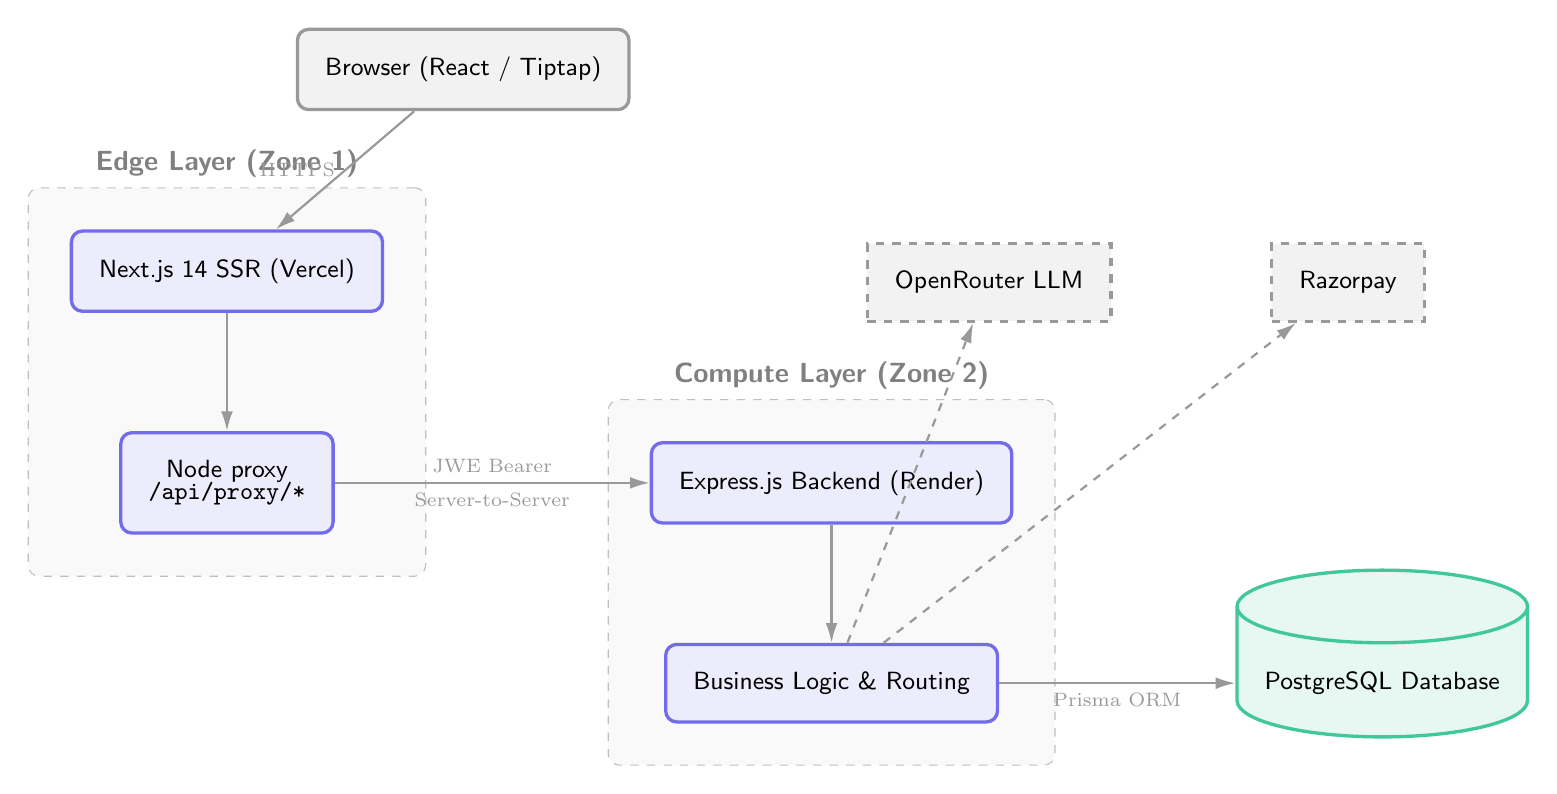
\begin{tikzpicture}[node distance=1.5cm and 2cm]
        
        % Client
        \node [component, fill=gray!10, draw=gray!80] (client) {Browser (React / Tiptap)};
        
        % Vercel Node
        \node [component, below=of client, xshift=-3cm] (vercel) {Next.js 14 SSR (Vercel)};
        \node [component, below=of vercel, align=center] (proxy) {Node proxy\\[-3pt]\texttt{/api/proxy/*}};
        
        \begin{scope}[on background layer]
            \node [groupbox, fit=(vercel) (proxy)] (vercelgroup) {};
            \node [above, font=\sffamily\bfseries, color=gray] at (vercelgroup.north) {Edge Layer (Zone 1)};
        \end{scope}

        % Render Node
        \node [component, right=of proxy, xshift=2cm] (express) {Express.js Backend (Render)};
        \node [component, below=of express] (services) {Business Logic \& Routing};
        
        \begin{scope}[on background layer]
            \node [groupbox, fit=(express) (services)] (rendergroup) {};
            \node [above, font=\sffamily\bfseries, color=gray] at (rendergroup.north) {Compute Layer (Zone 2)};
        \end{scope}

        % Database
        \node [database, right=of services, xshift=1cm] (db) {PostgreSQL Database};

        % External APIs
        \node [external, above=of express, xshift=2cm] (llm) {OpenRouter LLM};
        \node [external, right=of llm] (stripe) {Razorpay};

        % Connections
        \draw [line] (client) -- node[anchor=east, font=\scriptsize] {HTTPS} (vercel);
        \draw [line] (vercel) -- (proxy);
        \draw [line] (proxy) -- node[anchor=north, font=\scriptsize] {Server-to-Server} node[anchor=south, font=\scriptsize] {JWE Bearer} (express);
        \draw [line] (express) -- (services);
        \draw [line] (services) -- node[anchor=north, font=\scriptsize] {Prisma ORM} (db);
        
        \draw [line, dashed] (services) -- (llm);
        \draw [line, dashed] (services) -- (stripe);

    \end{tikzpicture}
    \caption{Macro-Level Decoupled Systems Architecture}
    \label{fig:macro_arch}
\end{figure}

\section{Technological Justifications}
\begin{itemize}[leftmargin=*]
    \item \textbf{Express.js over Next.js API Routes:} Generating an academic citation or rewriting 3,000 words via an LLM often exceeds the 10-second serverless timeout imposed by platforms like Vercel. Extracting this to a long-lived Node.js Express process ensures TCP sockets remain open for data streaming and heavy concurrent processing.
    \item \textbf{Prisma ORM over Raw SQL:} Managing 21 highly relational tables representing RBAC teams, documents, revisions, and audits requires mathematical precision. Prisma provides static \texttt{type} verification up to the repository boundary layer, completely eliminating runtime \texttt{TypeError} failures common in raw SQL mapping.
\end{itemize}

% -----------------------------------------------------------
% Chapter 3
% -----------------------------------------------------------
\chapter{Zero-Leakage Security Model}

\section{Cross-Domain Session Proxying}
Modern browsers enforce rigorous Cross-Site Request Forgery (CSRF) and cookie policies, predominantly blocking `SameSite=Lax` or `Strict` cookies from attaching to requests sent across distinct domains (\textit{wordsage.vercel.app} to \textit{wordsage-l10x.onrender.com}). 

To mitigate this without disabling browser security headers, WordSage implements the \textbf{Next-Auth Proxy Bridge}:

\begin{figure}[H]
    \centering
    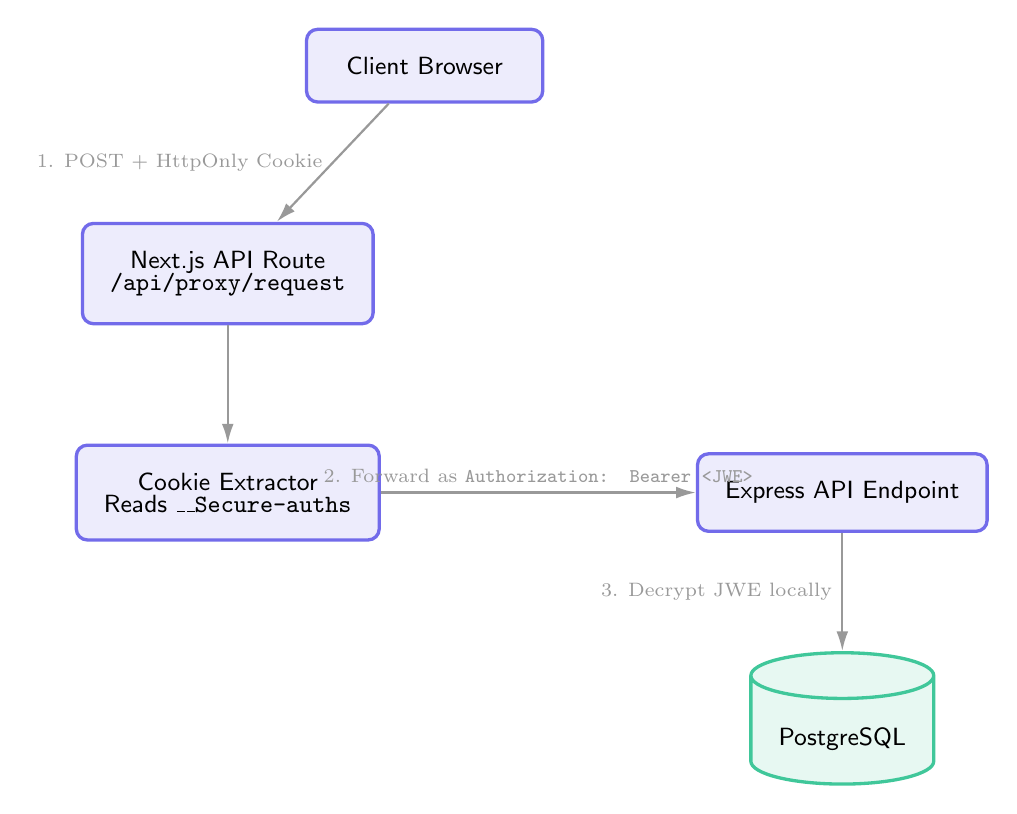
\begin{tikzpicture}[node distance=1.5cm and 2cm]
        
        \node [component, minimum width=3cm] (browser) {Client Browser};
        
        \node [component, below=of browser, xshift=-2.5cm, align=center] (api) {Next.js API Route\\[-3pt]\texttt{/api/proxy/request}};
        
        \node [component, below=of api, align=center] (extractor) {Cookie Extractor\\[-3pt]Reads \texttt{\_\_Secure-auths}};
        
        \node [component, right=of extractor, xshift=2cm] (backend) {Express API Endpoint};
        
        \node [database, below=of backend] (db) {PostgreSQL};

        % Paths
        \draw [line] (browser) -- node[anchor=east, font=\scriptsize] {1. POST + HttpOnly Cookie} (api);
        \draw [line] (api) -- (extractor);
        \draw [line] (extractor) -- node[anchor=south, font=\scriptsize] {2. Forward as \texttt{Authorization: Bearer <JWE>}} (backend);
        \draw [line] (backend) -- node[anchor=east, font=\scriptsize] {3. Decrypt JWE locally} (db);
        
    \end{tikzpicture}
    \caption{The Zero-Leakage Proxy Authentication Flow}
    \label{fig:auth_flow}
\end{figure}

\subsection{Implementation Detail}
By keeping the session cookie mapped to the Vercel domain, the browser naturally attaches it. The Vercel server, acting as a trusted entity, reads this cookie, extracts the raw JSON Web Encryption (JWE) string, calculates the requisite derivation salt, and injects it as an HTTP \texttt{Authorization} header payload sent to the Express backend. At no point is the \texttt{localStorage} capable of accessing the session.

\section{Secure Password Reset Sequence}
WordSage rejects naive UUID v4 resets. The implementation uses:
\begin{enumerate}
    \item \textbf{Disposable Domain Screening:} An in-memory Hash Set blocks requests from over 400 known temporary email providers (e.g., \textit{10minutemail}).
    \item \textbf{Cryptographic Token Generation:} Produced natively via \texttt{crypto.randomBytes(64).toString('hex')}.
    \item \textbf{Failover Obfuscation:} The API universally returns `HTTP 200 OK` whether the email exists or not, neutralizing attacker enumeration telemetry.
\end{enumerate}

% -----------------------------------------------------------
% Chapter 4
% -----------------------------------------------------------
\chapter{AI Inference \& Constraints Engine}

WordSage is not a simple proxy to OpenAI. It is an \textit{enforced pipeline}. Enterprise users require determinism; WordSage applies programmatic constraints to LLM generation.

\begin{figure}[H]
    \centering
    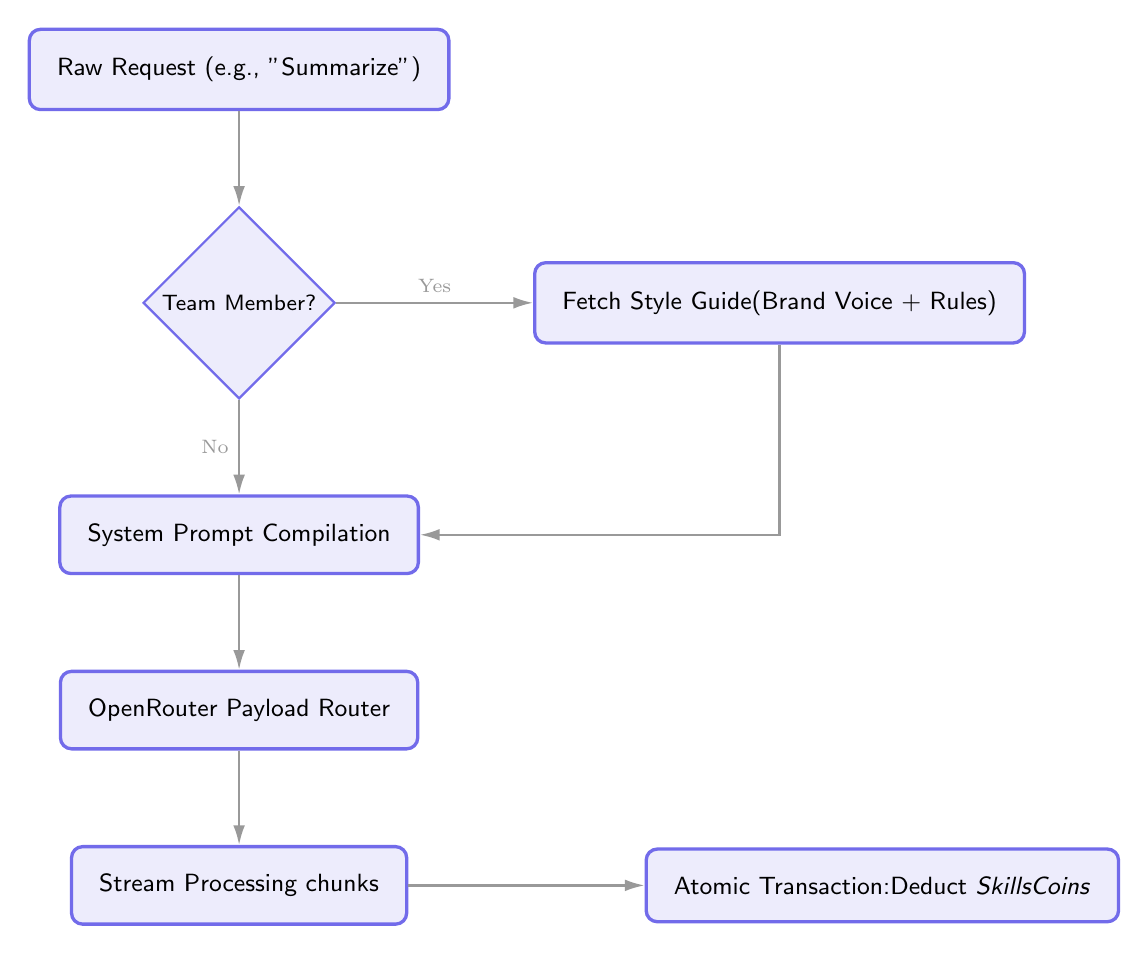
\begin{tikzpicture}[node distance=1.2cm and 1cm]
        
        \node [component] (input) {Raw Request (e.g., "Summarize")};
        
        \node [diamond, draw=primary!80, fill=primary!10, thick, text centered, inner sep=2pt, below=of input, font=\sffamily\footnotesize] (team) {Team Member?};
        
        \node [component, right=of team, xshift=1.5cm] (style) {Fetch Style Guide\\(Brand Voice + Rules)};
        
        \node [component, below=of team] (compile) {System Prompt Compilation};
        
        \node [component, below=of compile] (gateway) {OpenRouter Payload Router};
        
        \node [component, below=of gateway] (stream) {Stream Processing chunks};
        
        \node [component, right=of stream, xshift=2cm] (ledger) {Atomic Transaction:\\Deduct \textit{SkillsCoins}};

        % Draws
        \draw [line] (input) -- (team);
        \draw [line] (team) -- node[anchor=south, font=\scriptsize] {Yes} (style);
        \draw [line] (team) -- node[anchor=east, font=\scriptsize] {No} (compile);
        \draw [line] (style) |- (compile);
        \draw [line] (compile) -- (gateway);
        \draw [line] (gateway) -- (stream);
        \draw [line] (stream) -- (ledger);
        
    \end{tikzpicture}
    \caption{The Enforced AI Execution Pipeline}
    \label{fig:ai_flow}
\end{figure}

Prior to execution, if a user operates within an RBAC Team Context, the backend autonomously queries the \texttt{team\_style\_guides} table. Variables such as \textit{``Forbidden Terms: [synergy, leverage]''} and \textit{``Voice: Authoritative but approachable''} are synthesized into the LangChain-style system prompt instructing the model to reject inputs breaking corporate guidelines.

% -----------------------------------------------------------
% Chapter 5
% -----------------------------------------------------------
\chapter{The Financial Consensus Ledger}

\section{The Virtual Economy (\textit{SkillsCoins})}
Handling virtual currency demands financial-grade precision. WordSage utilizes a localized double-entry ledger design mapping. Every subtraction of coins related to AI usage and every addition related to Razorpay subscriptions are written permanently to the \texttt{coins\_transactions} table.

\subsection{Atomic Transactions}
To effectively halt ``Double Spend'' race conditions where a user clicks "Generate" rapidly twenty times with a low balance, the charge event is wrapped aggressively in Prisma isolated transactions:

\begin{lstlisting}[language=JavaScript, caption=Atomic Ledger Insertion Strategy]
await prisma.$transaction(async (tx) => {
    // 1. Verify exact balance locked
    const profile = await tx.user_profiles.findUnique({...});
    if (profile.coins < COST) throw new Error("Insufficient");
    
    // 2. Perform Deduction
    await tx.user_profiles.update({ 
        data: { coins: { decrement: COST } } 
    });
    
    // 3. Write Immutable Ledger Entry
    await tx.coins_transactions.create({
        data: { amount: -COST, type: "USAGE" }
    });
});
\end{lstlisting}

\section{Cryptographic Webhook Resolution}
Razorpay triggers asynchronous hooks signalling successful payments. These network hits are fundamentally untrusted until WordSage reconstructs the \texttt{HMAC-SHA256} digest over the raw unparsed request buffer against the \texttt{RAZORPAY\_WEBHOOK\_SECRET}. Only computationally identical hashes unlock database modifications.

% -----------------------------------------------------------
% Chapter 6
% -----------------------------------------------------------
\chapter{Deployment \& Orchestration}

WordSage ships with a \texttt{docker-compose.yml} configuration designed for immediate instantiation of the complete ecosystem within secure VLANs if cloud-platform decoupling is unnecessary.

\begin{itemize}
    \item \textbf{Ingress Controller:} Nginx acting as a Layer 7 Reverse Proxy.
    \item \textbf{Graceful Degradation:} The Express backend binds to POSIX signals (\texttt{SIGTERM / SIGINT}) to drain operating connections and flush outstanding analytical telemetry arrays before exiting.
    \item \textbf{Stateless Execution:} The Node.js layer holds zero state matrices, allowing horizontal scaling behind Kubernetes ReplicaSets.
\end{itemize}

\end{document}
